\section{Evaluation}
\label{sec:evaluation}

All the results presented in this sections are obtained with a test set containing the examples from $3001$ to $5000$.

\subsection{Training Error}
\begin{figure}[t]
	\centering
	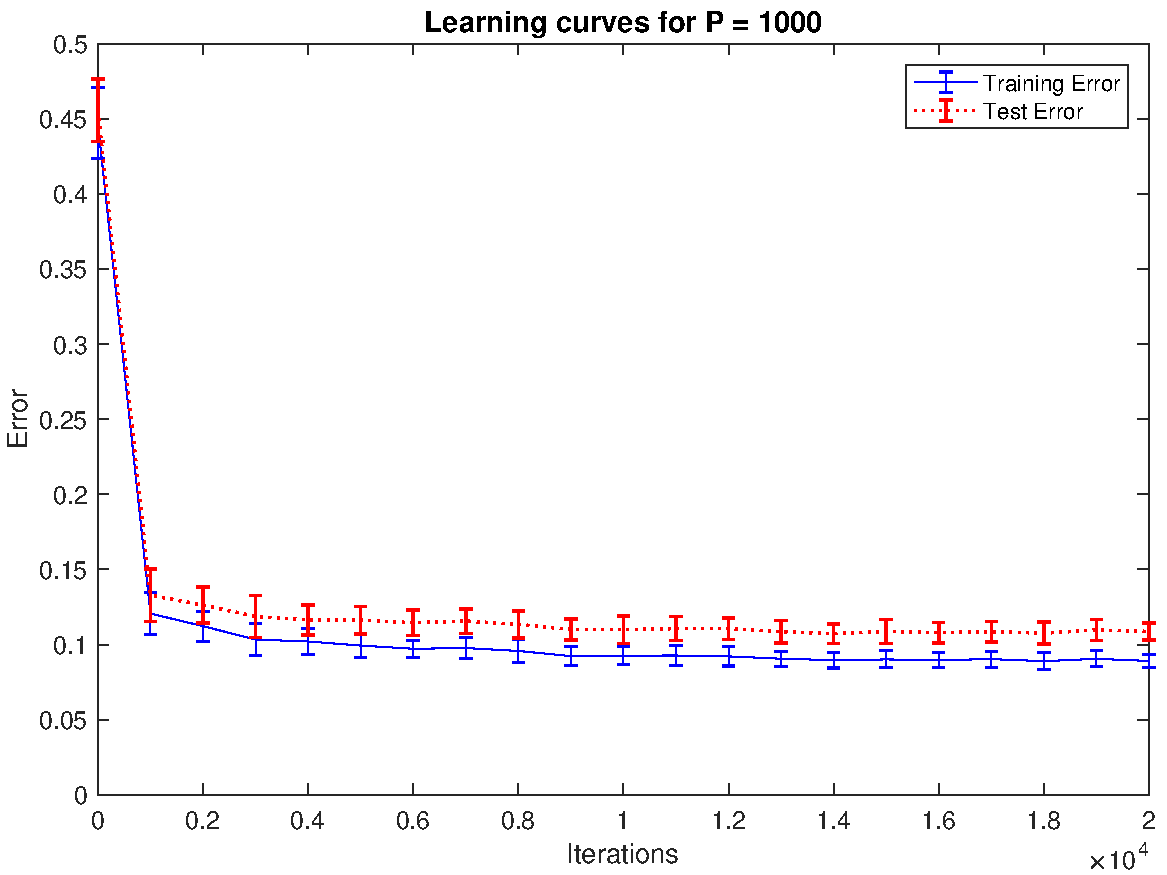
\includegraphics[width=\columnwidth]{figures/error}
    \caption{Training and test error of the network for $P = 1000$.}
	\label{fig:training_error}
\end{figure}

\cref{fig:training_error} shows the train and test error for the network trained using Stochastic Gradient Descent on the first $1000$ examples.
Both the train error and test error drop very quickly during approximately the first $1000$ iterations, then remain almost constant for the rest of the training.
The test error is slightly bigger than the train error:
at the end of the training, the train error is around $0.10$ and the test error around $0.12$.
Since the test error never increases, the model does not seem to overfit the training data.

\subsection{Learned Weights}
\begin{figure}[t]
	\centering
	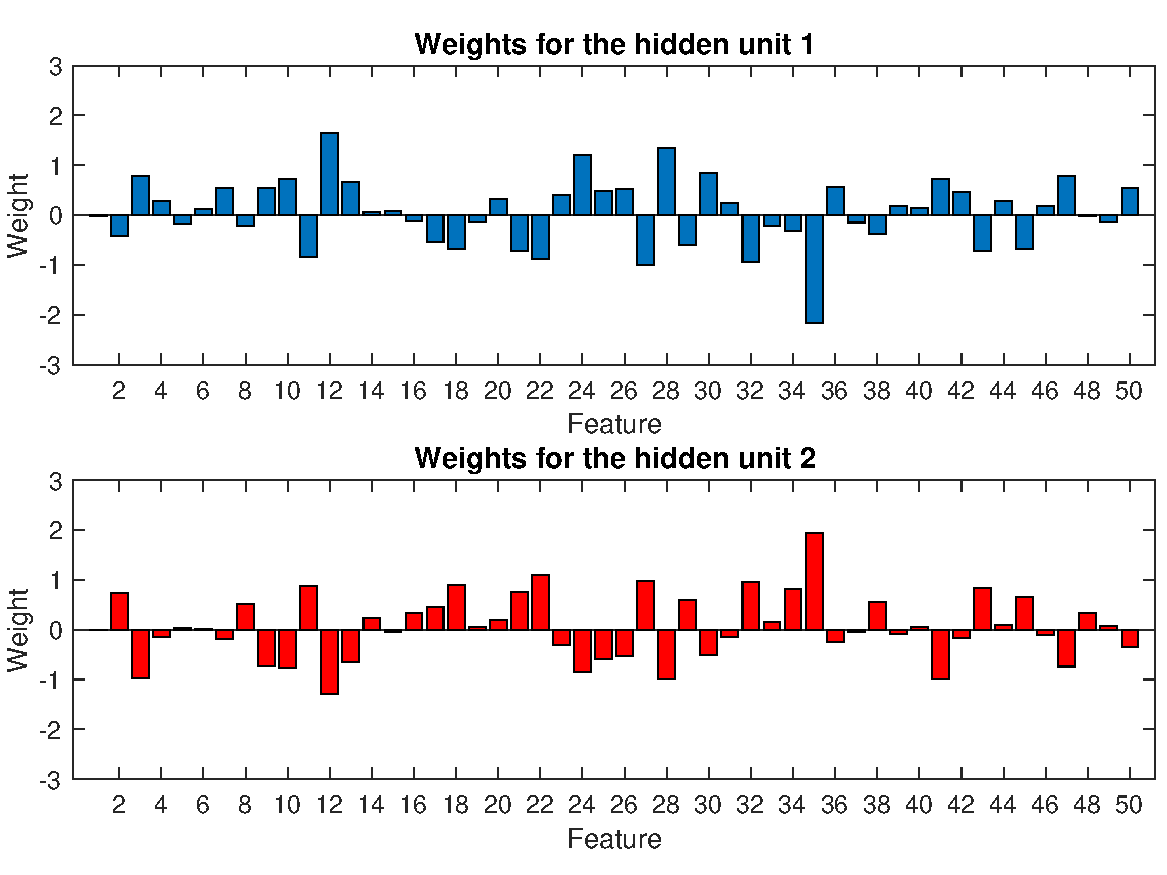
\includegraphics[width=\columnwidth]{figures/weights_p_1000}
    \caption{Weights of the hidden units of the network after the training.}
	\label{fig:weights}
\end{figure}

\cref{fig:weights} shows the weights learned from the hidden units of the networks after the training for $P = 1000$.
As expected, the units learn different weights thanks to the random initialization of the weights.
It is important ...

\subsection{Training Dataset}

\subsection{Training Policy}
